% Schematic of the toy model behind examples/square_lattice_toy.py and the Toy page.
% Build: npm run schematic  (python3 scripts/toy_schematic.py)
%   -> site/results/toy-schematic.{pdf,svg,png}
% Needs pdflatex with the standalone class and TikZ (on Banff: TinyTeX in ~/.TinyTeX).
%
% Every number in the figure is a property of the code:
%   lattice 121 x 121, open edges, K = M = 1 (phdef.models.square_lattice_dynmat);
%   cluster = Manhattan ball |i|+|j| <= 2, 13 sites (phdef.models.manhattan_partition);
%   D_bc: 20 springs from the 8 sites at |i|+|j| = 2 to the 12 at |i|+|j| = 3, rank 8;
%   first Lanczos block Q_1 lives on the shell |i|+|j| = 3, Q_2 on |i|+|j| = 4;
%   block j reaches |i|+|j| = 2 + j; dim Ct = 13 + 8 m (m = 160: 1293).
\documentclass[border=5pt]{standalone}
\usepackage[T1]{fontenc}
\usepackage{lmodern}
\usepackage{amsmath,amssymb}
\usepackage{tikz}
\usetikzlibrary{decorations.pathmorphing,decorations.pathreplacing}
% Reproducible PDF: no dates, no trailer id, no pdfTeX info.
\ifdefined\pdftrailerid \pdftrailerid{}\fi
\ifdefined\pdfinfoomitdate \pdfinfoomitdate=1\fi
\ifdefined\pdfsuppressptexinfo \pdfsuppressptexinfo=-1\fi

% Same colours as scripts/toy_figures.py: neutral inks, the validated blue ramp
% (#86b6ef, #2a78d6, #104281) and the categorical orange #eb6834.
\definecolor{ink}{HTML}{0B0B0B}
\definecolor{ink2}{HTML}{52514E}
\definecolor{muted}{HTML}{898781}
\definecolor{rule}{HTML}{C3C2B7}
\definecolor{tint}{HTML}{E1E0D9}
\definecolor{defect}{HTML}{EB6834}
\definecolor{defecttext}{HTML}{B4461A}
\definecolor{blueD}{HTML}{104281}
\definecolor{blueM}{HTML}{2A78D6}
\definecolor{blueL}{HTML}{86B6EF}

\tikzset{
  spring/.style={decorate, decoration={zigzag, segment length=1.2mm, amplitude=0.48mm,
                 pre length=1.7mm, post length=1.7mm}},
  host/.style={spring, draw=muted, line width=0.4pt},
  kprime/.style={spring, draw=defect, line width=1.0pt},
  dbc/.style={spring, draw=blueD, line width=0.9pt},
  stub/.style={draw=rule, line width=0.5pt, dash pattern=on 0.7pt off 1.1pt},
  title/.style={anchor=base west, font=\normalsize, text=ink},
  subtitle/.style={anchor=base west, font=\footnotesize, text=ink2},
  legend/.style={anchor=base west, font=\footnotesize, text=ink, inner sep=0pt},
  block/.style={draw=white, line width=0.6pt},
  blocklabel/.style={font=\scriptsize, inner sep=0pt},
}

% site markers, by Manhattan distance from the defect
\newcommand{\defectsite}[1]{\fill[defect] #1 circle (0.15); \draw[white, line width=0.6pt] #1 circle (0.15);}
\newcommand{\clustersite}[1]{\fill[blueD] #1 circle (0.095);}
\newcommand{\boundarysite}[1]{\filldraw[fill=white, draw=blueD, line width=0.55pt] #1 circle (0.155); \fill[blueD] #1 circle (0.08);}
\newcommand{\qonesite}[1]{\fill[blueM] #1 circle (0.09);}
\newcommand{\qtwosite}[1]{\filldraw[fill=blueL, draw=blueM, line width=0.3pt] #1 circle (0.09);}
\newcommand{\bathsite}[1]{\fill[muted] #1 circle (0.07);}

\begin{document}
\pagecolor{white}
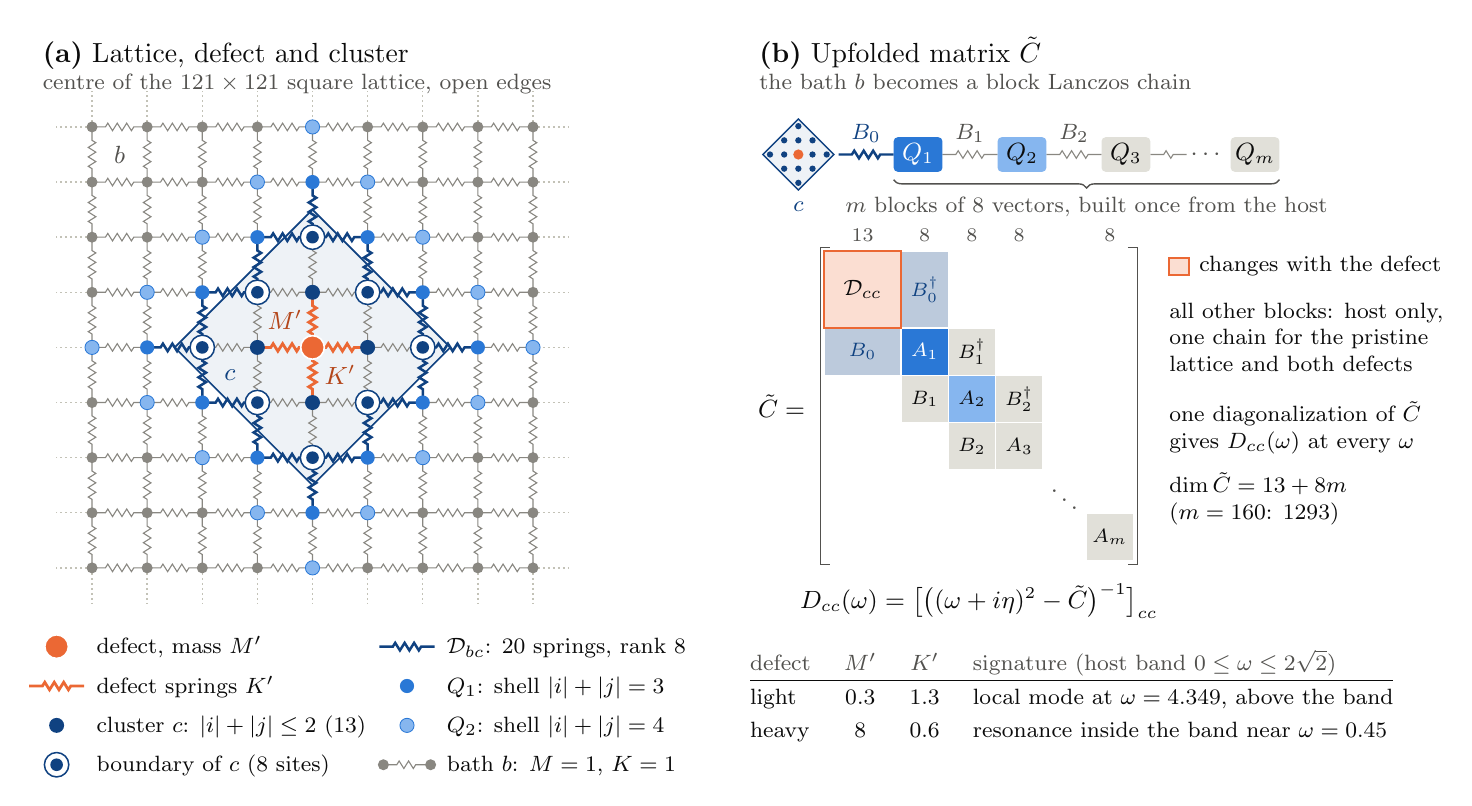
\begin{tikzpicture}[x=1cm, y=1cm, font=\small, text=ink]
\def\s{0.70}   % lattice constant in cm (bond = 3 zigzags of 1.2 mm)

% ======================= (a) real-space lattice =======================
\fill[blueD!7] (2.5*\s,0) -- (0,2.5*\s) -- (-2.5*\s,0) -- (0,-2.5*\s) -- cycle;
\draw[blueD, line width=0.6pt] (2.5*\s,0) -- (0,2.5*\s) -- (-2.5*\s,0) -- (0,-2.5*\s) -- cycle;

% the lattice continues beyond the window
\foreach \ii in {-4,...,4} {
  \draw[stub] (4*\s,\ii*\s) -- (4.65*\s,\ii*\s);
  \draw[stub] (-4*\s,\ii*\s) -- (-4.65*\s,\ii*\s);
  \draw[stub] (\ii*\s,4*\s) -- (\ii*\s,4.65*\s);
  \draw[stub] (\ii*\s,-4*\s) -- (\ii*\s,-4.65*\s);
}

% springs: defect bonds (shell 0-1), D_bc (shell 2-3), host otherwise
\foreach \x in {-4,...,4} {
  \foreach \y in {-4,...,4} {
    \pgfmathtruncatemacro{\dd}{abs(\x)+abs(\y)}
    \ifnum\x<4
      \pgfmathtruncatemacro{\lo}{min(\dd,abs(\x+1)+abs(\y))}
      \ifnum\lo=0 \draw[kprime] (\x*\s,\y*\s) -- (\x*\s+\s,\y*\s);
      \else\ifnum\lo=2 \draw[dbc] (\x*\s,\y*\s) -- (\x*\s+\s,\y*\s);
      \else \draw[host] (\x*\s,\y*\s) -- (\x*\s+\s,\y*\s);
      \fi\fi
    \fi
    \ifnum\y<4
      \pgfmathtruncatemacro{\lo}{min(\dd,abs(\x)+abs(\y+1))}
      \ifnum\lo=0 \draw[kprime] (\x*\s,\y*\s) -- (\x*\s,\y*\s+\s);
      \else\ifnum\lo=2 \draw[dbc] (\x*\s,\y*\s) -- (\x*\s,\y*\s+\s);
      \else \draw[host] (\x*\s,\y*\s) -- (\x*\s,\y*\s+\s);
      \fi\fi
    \fi
  }
}

% sites
\foreach \x in {-4,...,4} {
  \foreach \y in {-4,...,4} {
    \pgfmathtruncatemacro{\dd}{abs(\x)+abs(\y)}
    \ifcase\dd \defectsite{(\x*\s,\y*\s)}
    \or \clustersite{(\x*\s,\y*\s)}
    \or \boundarysite{(\x*\s,\y*\s)}
    \or \qonesite{(\x*\s,\y*\s)}
    \or \qtwosite{(\x*\s,\y*\s)}
    \else \bathsite{(\x*\s,\y*\s)}
    \fi
  }
}

% direct labels
\node[text=defecttext] at (-0.5*\s,0.5*\s) {$M'$};
\node[text=defecttext] at (0.5*\s,-0.5*\s) {$K'$};
\node[text=blueD] at (-1.5*\s,-0.5*\s) {$c$};
\node[text=ink2] at (-3.5*\s,3.5*\s) {$b$};

% title
\node[title] at (-3.55,3.62) {\textbf{(a)} Lattice, defect and cluster};
\node[subtitle] at (-3.55,3.27) {centre of the $121\times121$ square lattice, open edges};

% legend
\begin{scope}[shift={(-3.25,-3.80)}]
  \defectsite{(0,0)}                         \node[legend] at (0.5,-0.09) {defect, mass $M'$};
  \draw[kprime] (-0.35,-0.5) -- (0.35,-0.5); \node[legend] at (0.5,-0.59) {defect springs $K'$};
  \clustersite{(0,-1.0)}                     \node[legend] at (0.5,-1.09) {cluster $c$: $|i|+|j|\le2$ (13)};
  \boundarysite{(0,-1.5)}                    \node[legend] at (0.5,-1.59) {boundary of $c$ (8 sites)};
\end{scope}
\begin{scope}[shift={(1.20,-3.80)}]
  \draw[dbc] (-0.35,0) -- (0.35,0);          \node[legend] at (0.5,-0.09) {$\mathcal D_{bc}$: 20 springs, rank 8};
  \qonesite{(0,-0.5)}                        \node[legend] at (0.5,-0.59) {$Q_1$: shell $|i|+|j|=3$};
  \qtwosite{(0,-1.0)}                        \node[legend] at (0.5,-1.09) {$Q_2$: shell $|i|+|j|=4$};
  \draw[host] (-0.3,-1.5) -- (0.3,-1.5); \bathsite{(-0.3,-1.5)} \bathsite{(0.3,-1.5)}
                                             \node[legend] at (0.5,-1.59) {bath $b$: $M=1$, $K=1$};
\end{scope}

% ======================= (b) upfolded matrix =======================
\begin{scope}[shift={(5.55,0)}]
\node[title] at (0,3.62) {\textbf{(b)} Upfolded matrix $\tilde C$};
\node[subtitle] at (0,3.27) {the bath $b$ becomes a block Lanczos chain};

% --- chain picture ---
\def\cy{2.45}
\begin{scope}[shift={(0.62,\cy)}]
  \def\uu{0.18}
  \fill[blueD!7] (2.5*\uu,0) -- (0,2.5*\uu) -- (-2.5*\uu,0) -- (0,-2.5*\uu) -- cycle;
  \draw[blueD, line width=0.5pt] (2.5*\uu,0) -- (0,2.5*\uu) -- (-2.5*\uu,0) -- (0,-2.5*\uu) -- cycle;
  \foreach \x in {-2,...,2} {
    \foreach \y in {-2,...,2} {
      \pgfmathtruncatemacro{\dd}{abs(\x)+abs(\y)}
      \ifnum\dd=0 \fill[defect] (\x*\uu,\y*\uu) circle (0.065);
      \else\ifnum\dd<3 \fill[blueD] (\x*\uu,\y*\uu) circle (0.04);\fi\fi
    }
  }
\end{scope}
\draw[dbc] (1.13,\cy) -- (1.83,\cy);
\draw[host] (2.45,\cy) -- (3.15,\cy);
\draw[host] (3.77,\cy) -- (4.47,\cy);
\draw[host] (5.09,\cy) -- (5.55,\cy);
\node[font=\footnotesize, text=blueD] at (1.48,\cy+0.27) {$B_0$};
\node[font=\footnotesize, text=ink2] at (2.80,\cy+0.27) {$B_1$};
\node[font=\footnotesize, text=ink2] at (4.12,\cy+0.27) {$B_2$};
\node[font=\small, text=ink2] at (5.82,\cy) {$\cdots$};
\foreach \cx/\fc/\tc/\lab in {2.14/blueM/white/Q_1, 3.46/blueL/ink/Q_2, 4.78/tint/ink/Q_3, 6.42/tint/ink/Q_m} {
  \filldraw[fill=\fc, draw=none, rounded corners=1.5pt] (\cx-0.31,\cy-0.22) rectangle (\cx+0.31,\cy+0.22);
  \node[text=\tc, font=\small] at (\cx,\cy) {$\lab$};
}
\draw[decorate, decoration={brace, mirror, amplitude=3pt}, draw=ink2, line width=0.5pt]
  (1.83,\cy-0.32) -- (6.73,\cy-0.32);
\node[font=\footnotesize, text=ink2] at (4.28,\cy-0.66) {$m$ blocks of 8 vectors, built once from the host};
\node[font=\footnotesize, text=blueD] at (0.62,\cy-0.66) {$c$};

% --- block-tridiagonal matrix ---
\def\mx{0.95}   % left edge
\def\my{1.22}   % top edge
\def\cb{0.975}  % cluster block: 13 coordinates
\def\qb{0.600}  % chain block: 8 coordinates
\def\gp{0.55}   % gap for the dots
% block edges along the diagonal: b0 .. b6
\pgfmathsetmacro{\bA}{\cb}
\pgfmathsetmacro{\bB}{\cb+\qb}
\pgfmathsetmacro{\bC}{\cb+2*\qb}
\pgfmathsetmacro{\bD}{\cb+3*\qb}
\pgfmathsetmacro{\bE}{\cb+3*\qb+\gp}
\pgfmathsetmacro{\bF}{\cb+4*\qb+\gp}
\newcommand{\blk}[6]{% col0 col1 row0 row1 fill label
  \filldraw[block, fill=#5] (\mx+#1,\my-#3) rectangle (\mx+#2,\my-#4);
  \node[blocklabel] at (\mx+0.5*#1+0.5*#2,\my-0.5*#3-0.5*#4) {#6};}
\blk{0}{\bA}{0}{\bA}{defect!22}{\footnotesize$\mathcal D_{cc}$}
\blk{0}{\bA}{\bA}{\bB}{blueD!28}{\textcolor{blueD}{$B_0$}}
\blk{\bA}{\bB}{0}{\bA}{blueD!28}{\textcolor{blueD}{$B_0^{\dagger}$}}
\blk{\bA}{\bB}{\bA}{\bB}{blueM}{\textcolor{white}{$A_1$}}
\blk{\bA}{\bB}{\bB}{\bC}{tint}{$B_1$}
\blk{\bB}{\bC}{\bA}{\bB}{tint}{$B_1^{\dagger}$}
\blk{\bB}{\bC}{\bB}{\bC}{blueL}{$A_2$}
\blk{\bB}{\bC}{\bC}{\bD}{tint}{$B_2$}
\blk{\bC}{\bD}{\bB}{\bC}{tint}{$B_2^{\dagger}$}
\blk{\bC}{\bD}{\bC}{\bD}{tint}{$A_3$}
\blk{\bE}{\bF}{\bE}{\bF}{tint}{$A_m$}
\node[font=\small, text=ink2] at (\mx+0.5*\bD+0.5*\bE,\my-0.5*\bD-0.5*\bE) {$\ddots$};
\draw[defect, line width=0.8pt] (\mx,\my) rectangle (\mx+\bA,\my-\bA);
% matrix brackets and block sizes
\draw[ink2, line width=0.6pt] (\mx+0.07,\my+0.05) -- (\mx-0.05,\my+0.05) -- (\mx-0.05,\my-\bF-0.05) -- (\mx+0.07,\my-\bF-0.05);
\draw[ink2, line width=0.6pt] (\mx+\bF-0.07,\my+0.05) -- (\mx+\bF+0.05,\my+0.05) -- (\mx+\bF+0.05,\my-\bF-0.05) -- (\mx+\bF-0.07,\my-\bF-0.05);
\node[anchor=east] at (\mx-0.12,\my-0.5*\bF) {$\tilde C=$};
\foreach \pa/\pb/\n in {0/\bA/13, \bA/\bB/8, \bB/\bC/8, \bC/\bD/8, \bE/\bF/8}
  \node[font=\scriptsize, text=ink2, anchor=base] at (\mx+0.5*\pa+0.5*\pb,\my+0.12) {\n};

% --- notes to the right of the matrix ---
\begin{scope}[shift={(\mx+\bF+0.45,\my-0.05)}]
  \fill[defect!22] (0,-0.25) rectangle (0.26,-0.03); \draw[defect, line width=0.8pt] (0,-0.25) rectangle (0.26,-0.03);
  \node[legend, anchor=north west, align=left] at (0.38,0) {changes with the defect};
  \node[legend, anchor=north west, align=left] at (0,-0.6) {all other blocks: host only,\\ one chain for the pristine\\ lattice and both defects};
  \node[legend, anchor=north west, align=left] at (0,-1.85) {one diagonalization of $\tilde C$\\ gives $D_{cc}(\omega)$ at every $\omega$};
  \node[legend, anchor=north west, align=left] at (0,-2.75) {$\dim\tilde C=13+8m$\\ ($m=160$: 1293)};
\end{scope}

% --- formula and the two defects ---
\node[anchor=base, font=\small] at (\mx+0.5*\bF,-3.32)
  {$D_{cc}(\omega)=\big[\big((\omega+i\eta)^2-\tilde C\big)^{-1}\big]_{cc}$};
\node[anchor=north west, font=\footnotesize, inner sep=0pt] at (0,-3.80) {%
  \renewcommand{\arraystretch}{1.25}%
  \begin{tabular}{@{}lccl@{}}
    \textcolor{ink2}{defect} & \textcolor{ink2}{$M'$} & \textcolor{ink2}{$K'$} & \textcolor{ink2}{signature (host band $0\le\omega\le2\sqrt2$)}\\
    \hline
    light & 0.3 & 1.3 & local mode at $\omega=4.349$, above the band\\
    heavy & 8   & 0.6 & resonance inside the band near $\omega=0.45$\\
  \end{tabular}};
\end{scope}
\end{tikzpicture}
\end{document}
